%!TEX root=../main.tex
\chapter{Climbing Mont Blanc Improvements}
\label{ch:improvements}

In this chapter it is assumed that a web interface follows the \gls{mvc} pattern. As briefly mentioned in sub-section \ref{subsec:cmb-arch-frontend}, Angular structures the HTML and Javascript code according to the \gls{mvc} pattern, and the reader should have the abstraction in mind when reading about browser or frontend implementations.

\section{Real Time Updates}
The frontend view changes when a user performes actions against the frontend models as mentioned in sub-section \ref{subsec:cmb-arch-frontend}. However, the frontend view presented to a given user does not update automatically as other users interract and changes their data models, as models is stored locally in each of the user's browser. If the updated model contains data that should be known\footnote{Hereby known as \textit{shared data}.} to all users, the users does not get notified about the model changes dynamically and views may therefore display out of date information. Figure \ref{fig:update-problem} shows an example of the problem, as Alice updates some of her browser's model data when she interacts with the system. If Alice changes some data present in Bob's models, Bob will not be notified of the changes as all data transfer are done with HTTP requests between Alice and the server. However, Bob can fetch up to date data by manually refreshing his webpage. \\

\begin{sidewaysfigure}
    \centering
    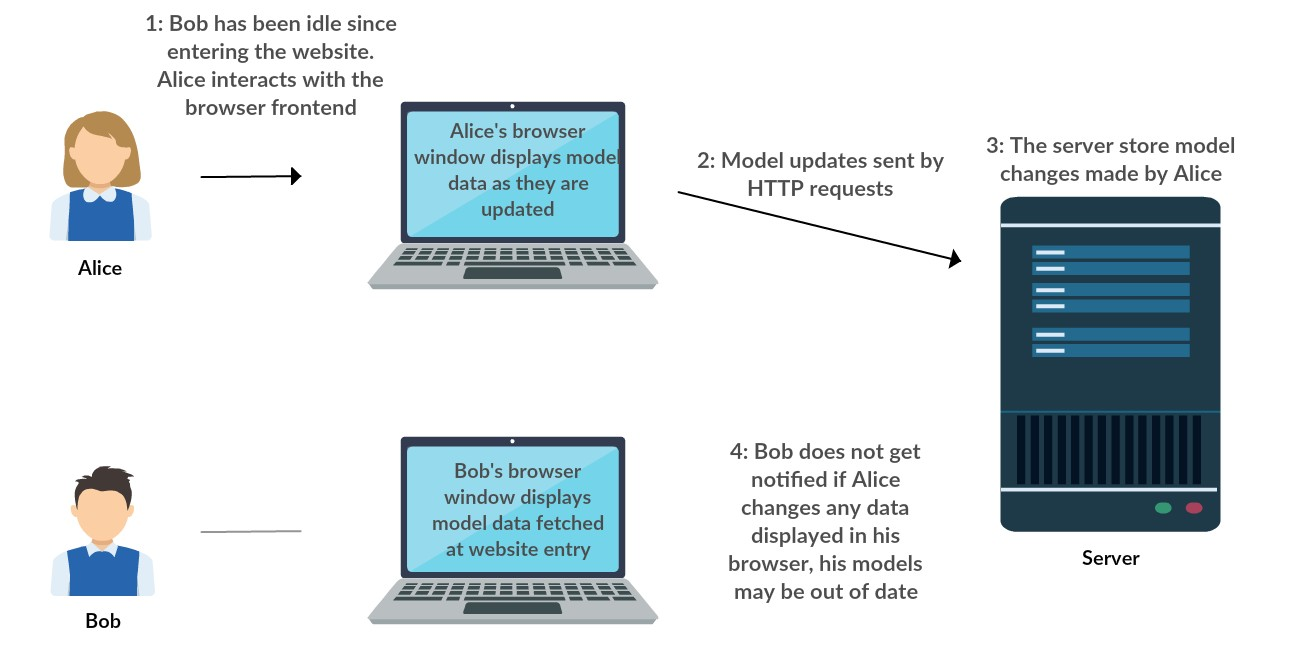
\includegraphics[width=1\textwidth]{figs/update_problem.jpg}
    \caption{Example of updating models without model change notifications}
    \label{fig:update-problem}
\end{sidewaysfigure}

Many websites requires to share data between multiple clients and dynamically notify clients if there are changes to the data. As an example in the \gls{cmb} system, it would be nice if the frontend interface dynamically updated as a user's submission finished running at the backend. In the old system before the improvements, the user had to manually refresh by clicking at a refresh button provided by the user interface or manually refresh the webpage. However, this section presents a technology which has been introduced in the new version of the system in order to dynamically update data relevant for multiple clients. \\

Socket.io \cite{SOCKETIO} is an \gls{api} for enabling real time communication between the server and connected clients. The \gls{api} was first made as Javascript library, but many open source projects have developed modules for other programming languages integrating the Socket.io \gls{api}. One benefit of the \gls{api} is that it works as a wrapper around a set of real time communication protocols to enable support for different browsers, which means that the framework can automatically detect the protocol supported by a client and use that information to select the best fitted communication protocol. \\

Rohit Rai states the communication protocols supported by the Socket.io \gls{api} \cite{Rai2013}. Figure \ref{fig:cmb-protocols} shows the communication protocols enabled in the new version of \gls{cmb}. The WebSocket protocol \cite{a:Fette2011}, shown in Figure \ref{fig:websocket}, has become more popular since its introduction in 2011 and is now supported by the most popular browsers. The protocol is a bit different from the well known HTTP protocol, as there is a persistent connection, or socket, between the client and the server as long as both entities are connected to the socket. The socket connection is closed if the client closes the browser window or the server goes down, or if the code explicitly indicates to close the socket. WebSockets enables easy two-way communication by letting two entities emit (read: send) messages back and forth on the socket connection, and respond differently depending on the type of message emitted on the socket. \\

Polling and long-polling are very similar as they both rely on the HTTP protocol. However, in long-polling, the server keeps the connection between the two entities open until there is an update to the requested data as shown in Figure \ref{fig:long-polling}. In polling, as shown in Figure \ref{fig:polling}, the client continously requests data with some constant delay between each request, while the server respond on each request with the data currently stored at the server. \\

Socket.io makes it easier for the programmer as well. The programmer does not need to worry about the functionality of the underlaying protocol, and can focus at writing code at high level of abstraction. Socket.io also enables the programmer to define their own \textit{events}, and have the \gls{api} listen for these events. If a given event is emitted (read:sent), and there . Both the server and client can set up listeners for events.

The two below sub-sections describes the changes done on the server and frontend code in order to support real time communication with Socket.io.

\begin{figure}
    \centering
    \begin{subfigure}[b]{1.0\textwidth}
        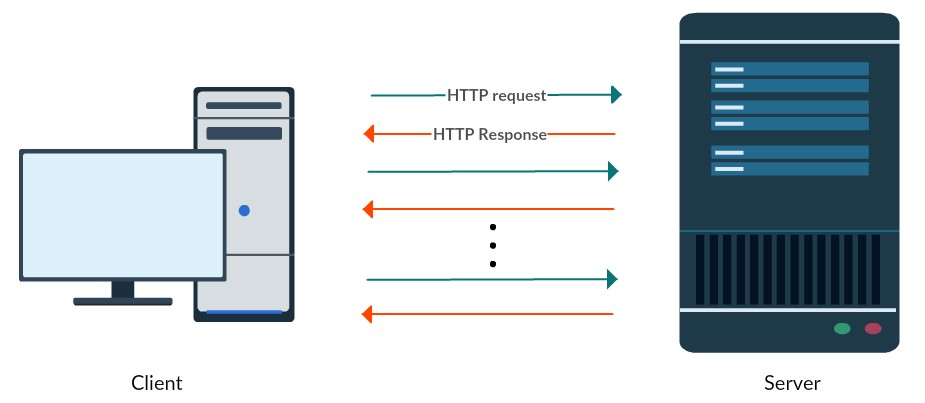
\includegraphics[width=\textwidth]{figs/polling.jpg}
        \caption{Polling: The client sends a series of HTTP request and the server responds on each request.}
        \label{fig:polling}
    \end{subfigure}
    ~ %add desired spacing between images, e. g. ~, \quad, \qquad, \hfill etc.
    %(or a blank line to force the subfigure onto a new line)
    \begin{subfigure}[b]{1.0\textwidth}
        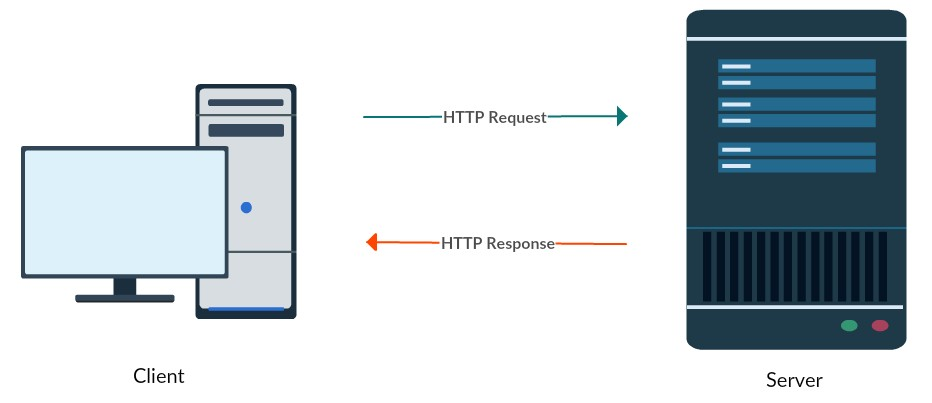
\includegraphics[width=\textwidth]{figs/long_polling.jpg}
        \caption{Long-polling: The client sends an HTTP request to fetch new data, the server holds the connection open until the requested data is updated.}
        \label{fig:long-polling}
    \end{subfigure}
    \begin{subfigure}[b]{1.0\textwidth}
        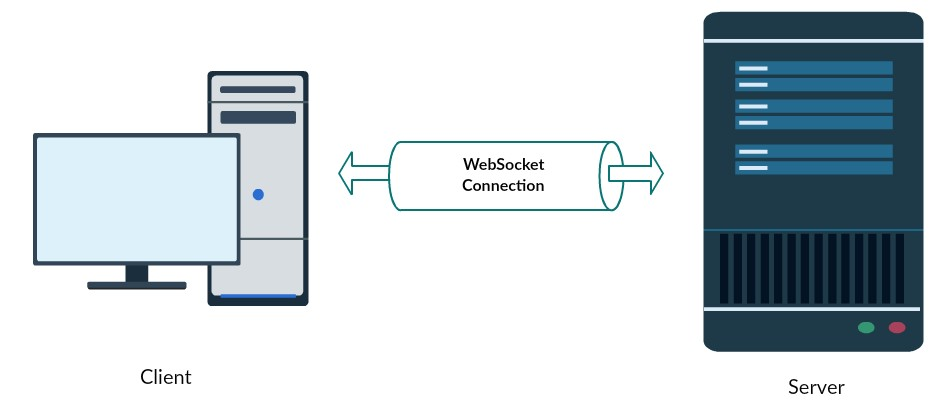
\includegraphics[width=\textwidth]{figs/websocket.jpg}
        \caption{WebSocket protocol: a two-way connection tunnel open throughout the whole client session. TCP is used as a transport protocol.}
        \label{fig:websocket}
    \end{subfigure}
    \caption{\gls{cmb} Socket.io communication protocols}\label{fig:cmb-protocols}
\end{figure}

\subsection{Frontend Changes}

\subsection{Server Changes}
The Python module Flask-SocketIO \cite{FLASKSOCKETIO} enables Flask applications to use the SocketIO \gls{api}. To support

\section{Frontend}
\subsection{Bug Fixes}
Upload fixes in frontend
Sorting bug

\subsection{Views and Feedback}
Spinners + better error messages. Bulletin board to display administrator messages.

\subsection{Group Functionality Improvements}
Moved

\section{Server}

\subsection{Database Management System}
SQLAlchemy MYSQL adapter + possible async library.

\subsection{Database Model Updates}
Detailed state field added and can be replaced with json structures as more information is needed about a run.

\subsection{Admin Interface}
Bug fix: Unix vs DOS files.
Cascading delete.

\section{Backend}
Some small changes needed to be done at the backend in order to improve the feedback given to the user


\section{Improvement Proposals}
